\begin{figure*}[t]
  \centering
  \begin{subfigure}[b]{0.58\textwidth}
    \centering
    \resizebox{\linewidth}{!}{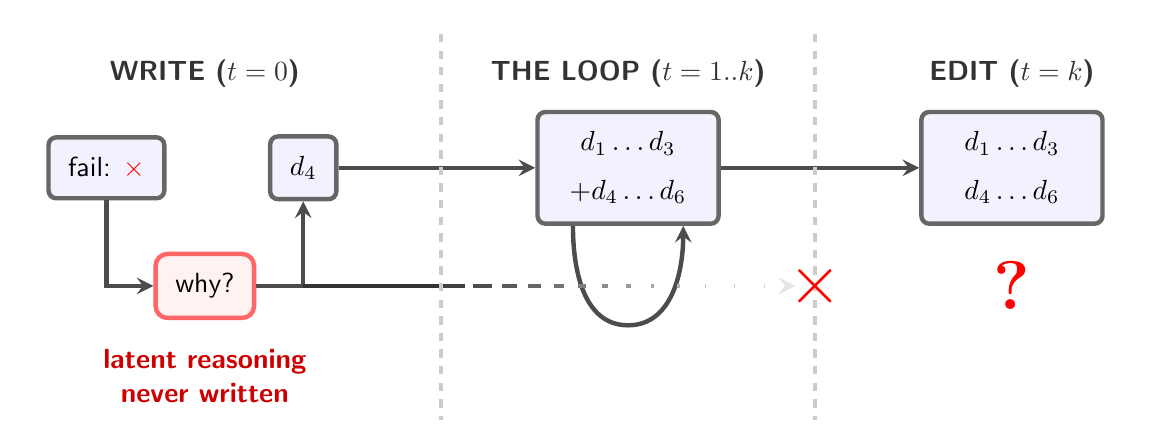
\begin{tikzpicture}[
    >=stealth,
    font=\sffamily,
    % Core styles: uniform standard font size, 1.6pt line widths (100% thicker)
    stage_title/.style={font=\sffamily\bfseries, text=black!80},
    mem/.style={draw=black!60, line width=1.6pt, rounded corners=1mm, fill=blue!5, align=center, inner sep=2.5mm},
    % why box explicitly defines the 2.5mm intra-box margin
    why/.style={draw=red!60, line width=1.6pt, rounded corners=1.5mm, fill=red!5, align=center, inner sep=2.5mm},
    ann/.style={font=\sffamily\bfseries, text=red!80!black, align=center},
    flow/.style={->, line width=1.6pt, draw=black!70}
  ]

  % Bounding box mathematically locked to 2.81 aspect ratio to prevent distortion (14 / 4.98)
  % Y=0.0 is precisely calibrated to match the header/box margin
  \useasboundingbox (0, 0) rectangle (14, 4.98);

  % ---------------------------------------------------------
  % PLANE 1: TEXT / TITLES (Y = 4.4)
  % ---------------------------------------------------------
  \node[stage_title] at (2.25, 4.4) {WRITE ($t=0$)};
  \node[stage_title] at (7.625, 4.4) {THE LOOP ($t=1..k$)};
  \node[stage_title] at (12.5, 4.4) {EDIT ($t=k$)};

  % ---------------------------------------------------------
  % PLANE 2: OBSERVABLES (Y = 3.2)
  % ---------------------------------------------------------
  \node[mem] (fail) at (1.0, 3.2) {fail: \textcolor{red}{\bfseries $\times$}};
  \node[mem] (d4) at (3.5, 3.2) {$d_4$};
  \node[mem, text width=1.8cm] (loopm) at (7.625, 3.2) {$d_1 \dots d_3$ \\ \vspace{2mm} $+d_4 \dots d_6$};
  \node[mem, text width=1.8cm] (readm) at (12.5, 3.2) {$d_1 \dots d_3$ \\ \vspace{2mm} $d_4 \dots d_6$};

  % Observable execution flows
  \draw[flow] (d4) -- (loopm);
  \draw[flow] (loopm) -- (readm);

  % ---------------------------------------------------------
  % PLANE 3: HIDDEN REASONING (Y = 1.7)
  % ---------------------------------------------------------
  \node[why] (why) at (2.25, 1.7) {why?};

  % Caption margin mathematically locked to exactly match the 2.5mm intra-box margin above
  \node[ann, anchor=north] at ([yshift=-2.5mm]why.south) {latent reasoning \\ never written};

  % Right-angled causal pathways
  \draw[flow] (fail.south) |- (why.west);
  \draw[flow] (why.east) -| (d4.south);

  % Depictive execution loop reaching deep into the reasoning plane (down to Y=1.2)
  \draw[flow] ([xshift=-0.7cm]loopm.south)
  to[out=270, in=180] (7.625, 1.2)
  to[out=0, in=270] ([xshift=0.7cm]loopm.south);

  % ---------------------------------------------------------
  % SMOOTH MANUAL DEGRADATION (X = 3.5 to X = 9.75)
  % ---------------------------------------------------------
  % Originates at the right-angle corner of the why->d4 arrow
  \draw[line width=1.6pt, draw=black!80] (3.5, 1.7) -- (5.25, 1.7); % Solid up to Write/Loop boundary

  % Exponentially decaying segment length, increasing gaps, and fading opacity
  \draw[line width=1.6pt, draw=black!75] (5.25, 1.7) -- (5.55, 1.7);
  \draw[line width=1.6pt, draw=black!70] (5.65, 1.7) -- (5.90, 1.7);
  \draw[line width=1.6pt, draw=black!65] (6.02, 1.7) -- (6.22, 1.7);
  \draw[line width=1.6pt, draw=black!60] (6.36, 1.7) -- (6.52, 1.7);
  \draw[line width=1.6pt, draw=black!55] (6.68, 1.7) -- (6.81, 1.7);
  \draw[line width=1.6pt, draw=black!50] (6.99, 1.7) -- (7.09, 1.7);
  \draw[line width=1.6pt, draw=black!45] (7.29, 1.7) -- (7.37, 1.7);
  \draw[line width=1.6pt, draw=black!40] (7.60, 1.7) -- (7.66, 1.7);
  \draw[line width=1.6pt, draw=black!35] (7.92, 1.7) -- (7.96, 1.7);
  \draw[line width=1.6pt, draw=black!30] (8.25, 1.7) -- (8.28, 1.7);
  \draw[line width=1.6pt, draw=black!25] (8.60, 1.7) -- (8.62, 1.7);
  \draw[line width=1.6pt, draw=black!20] (8.97, 1.7) -- (8.98, 1.7);
  \draw[line width=1.6pt, draw=black!15] (9.35, 1.7) -- (9.36, 1.7);
  \draw[->, line width=1.6pt, draw=black!10] (9.70, 1.7) -- (9.75, 1.7);

  % ---------------------------------------------------------
  % VERTICAL DIVIDERS AND BOUNDARY MARKERS
  % ---------------------------------------------------------
  \draw[dashed, black!20, line width=1.6pt] (5.25, 4.9) -- (5.25, 0.0);
  \draw[dashed, black!20, line width=1.6pt] (10.0, 4.9) -- (10.0, 0.0);

  % Degradation failure point exactly at the boundary (X=10.0)
  \node[text=red, font=\Huge\bfseries, inner sep=0pt] at (10.0, 1.7) {$\times$};

  % Read-time reasoning void
  \node[text=red, font=\Huge\bfseries] at (12.5, 1.7) {?};

\end{tikzpicture}
}
    \caption{
      Why do agentic prompts only grow? The latent reasoning behind $d_i$ is never written and decays over
      the (possibly agentic) development loop, so deletion risks an acute regression while the cost of
      addition stays diffuse.
    }
    \label{fig:flow}
  \end{subfigure}\hfill
  \begin{subfigure}[b]{0.38\textwidth}
    \centering
    \fbox{\parbox{0.96\linewidth}{\definecolor{synKey}{RGB}{135,0,175}
\definecolor{synMark}{RGB}{0,92,197}
\definecolor{synComment}{RGB}{0,128,0}
{\scriptsize\linespread{0.85}\selectfont\ttfamily\raggedright
  \textcolor{gray}{
    Write a brief post about how Earth is different from Venus.\\
    ...\\
    Write your response as three sentences, each ending with a period.
  }\textcolor{synComment}{\# Task 0 continues to fail on sentence count; last instruction was
  vague; maybe being explicit about periods will help?}\par
}
}}
    \caption{
      The fix: informative comments encode latent reasoning, which stops
      unbounded growth in agentic READMEs.
    }
    \label{fig:comment}
  \end{subfigure}
  \caption{
    The prompt-comment world. Latent reasoning is free at write-time and exponentially costly to reconstruct
    at read-time, but prompt comments preserve it and stop the unbounded growth of agentic READMEs.
  }
  \label{fig:comment_world}
\end{figure*}


\section{Introduction}
\label{sec:intro}

Overwhelmingly, agentic READMEs never stop growing. A \texttt{copilot-instructions.md},
\texttt{AGENTS.md} or \texttt{CLAUDE.md} gains instructions and rarely shed them
\citep{chatlatanagulchai2025agentreadmes}. Deleting the file is not the answer: repositories carrying one
finish agent tasks faster and in fewer tokens
\citep{lulla2026contextfiles}. Keeping everything is not free either: instruction-following degrades as
constraints accumulate \citep{jiang2024followbench, lior2025wildifeval}, and the median file already carries
\FieldOpMedian{} instructions, the average more than tripling over its own lifetime
(\FieldGrowthCountPeakPct{}, \autoref{fig:hero:growth}).

Different mechanisms can explain this growth. If requirements stop applying (instruction staleness), deletion
hazard rises with an instruction's age. If brittle instructions die young, leaving robust ones behind (content
fragility), hazard falls. If maintainers lose an instruction's rationale (imperfect recall), hazard falls
with age and, unlike either rival, also with the number of maintainers. Nobody has identified the root cause
because line diffs and file sizes cannot resolve individual instructions over time.

``What's the point of this code?'' is a question every engineer has asked. Deleting agentic
instructions risks a regression, and doing so safely requires counterfactuals that maintainers cannot
feasibly run. Recording an instruction's latent reasoning costs $O(1)$, but reconstructing
it costs $O(2^{|D|})$ for a prompt with $|D|$ instructions (\autoref{sec:theory}). Successive edits by
multiple authors destroy that latent reasoning, so deletion hazard decays with age, additions outrun
removals, and instructions grow without bound until agents become non-functional --- \textbf{catastrophic
remembering}. Under catastrophic forgetting, a gradient learner overwrites what it should have kept
\citep{mccloskey1989catastrophic, french1999catastrophic, kirkpatrick2017overcoming}; under catastrophic
remembering, a maintainer keeps what they should have overwritten. Both fail and fail for the same reason:
whatever would license the update is gone.\looseness=-1

How deletions actually occur in agentic prompts points to the root cause. \RewriteDeathShare{} of instruction
deaths arrive in one commit that bulldozes the file, after which growth resumes at its prior rate
(\autoref{sec:rewrite}): removing one instruction needs a reason, removing all needs none. And the hazard agrees
--- removal becomes less likely the older an instruction is, and less likely still the more authors have
edited the file (\autoref{sec:field}).

Software engineering solved this decades ago with the comment: text addressed to the next maintainer and
invisible to the interpreter \citep{knuth1984literate}. Recovering why code was written as it was is
developers' most serious problem \citep{latoza2006mentalmodels}, so the practice is to record the why, not
the how or the what \citep{mcconnell2004codecomplete}. Unsurprisingly, both carry over to agentic prompts.

We show that prompt comments encoding an instruction's latent reasoning can halt unbounded prompt growth,
removing \HorizonExcessRemovedPct{} of the excess size (\HorizonControlExcessPct{} to
\HorizonPracticalExcessPct{}) over \HorizonT{} steps, and cutting it from \LabControlExcessPct{} to
\LabPracticalExcessPct{} (\LabPracticalDeltaExcessPp{}) over \LabT{} (\autoref{fig:hero:lab}).
Because irrelevant context distracts models \citep{shi2023distracted}, this improves instruction-following on
real prompts by as much as \WildDeltaSatPct{} (\WildDeltaSatPp{}).
We ablate the effect across comment payloads to show outcome-grounded latent reasoning drives the gain.
Finally, we show that prompt comments' advantage only grows as (agentic) maintainers grow more capable
(\autoref{sec:lab}).\looseness=-1

We contribute a new approach to prompt maintenance, characterized across four dimensions:
\begin{itemize}[nosep,itemsep=2pt,parsep=2pt,topsep=2pt,leftmargin=*]
  \item \emph{Theory of prompt maintenance.} Decaying recoverability of latent reasoning predicts unbounded
    growth (\autoref{sec:theory}).
  \item \emph{Root cause of unbounded prompt growth.} Deletion hazard decays with age over \FieldSpells{}
    lifetimes, implicating imperfect recall, not instruction staleness or content fragility
    (\autoref{sec:hazard}).
  \item \emph{New evaluation with known optimum.} Inverting IFEval yields verifiable worlds whose minimum cover is
    known, so excess size and correctness become measurable (\autoref{sec:testbed}, \autoref{sec:wild}).
  \item \emph{Practical solution.} Prompt comments remove \HorizonExcessRemovedPct{} of the excess size
    (\autoref{sec:lab}), and improve instruction-following on real prompts by as much as \WildDeltaSatPct{}
    (\autoref{sec:wild}).
\end{itemize}
